\chapter{Resultados e Discussões} \label{cap:04}

Esta seção apresenta a análise aprofundada dos experimentos realizados durante o desenvolvimento do protótipo. Foram empregados testes quantitativos e qualitativos com o objetivo de comparar três modelos de IA para a tarefa de descrição de imagens. Para tanto, o \textit{benchmark} abrangeu métricas de latência, qualidade textual (utilizando BERTScore e ROUGE-L) e testes manuais, de forma a avaliar a coerência e a utilidade das descrições geradas. Em seguida, realiza-se uma análise crítica dos resultados, destacando os \textit{trade-offs} encontrados, e, finalmente, são discutidas as principais limitações do sistema desenvolvido.

\section{Resultados do \textit{Benchmark}}

Nesta seção, são apresentados e discutidos os resultados dos testes de \textit{benchmark} desenvolvidos para comparar os modelos escolhidos, com o objetivo de definir qual deles é o mais adequado para a construção do protótipo assistivo. Os experimentos quantitativos foram conduzidos utilizando o \textit{dataset} público \lstinline{coco-captions-pt-br} \cite{bromonschenkel2024cocopt}, que reúne imagens de diversos cenários – desde composições simples até ambientes com alta complexidade visual. Para cada modelo, foram coletadas as seguintes métricas:

\begin{itemize}
    \item \textbf{Latência:} Tempo médio, mediano e desvio padrão (em segundos) medindo o intervalo entre o envio da imagem para a API e o recebimento da descrição.
    \item \textbf{BERTScore:} Métrica que avalia a similaridade semântica entre a descrição gerada e as legendas de referência. A pontuação varia de 0 a 1, onde 0 indica nenhuma similaridade semântica entre os textos e 1 representa uma correspondência perfeita, considerando a proximidade de significado entre as palavras e suas representações contextuais.
    \item \textbf{ROUGE-L:} Índice que analisa a sobreposição lexical, mensurando a maior sequência comum de palavras entre o texto gerado e o de referência. Seu valor também varia de 0 a 1, onde 0 significa que não há palavras em comum entre os textos e 1 indica que o texto gerado é idêntico à referência em termos de estrutura lexical.
\end{itemize}

Essas métricas permitem uma avaliação integrada, capturando tanto a qualidade textual das descrições quanto o desempenho em termos de velocidade de processamento de cada modelo. 

Na Tabela \ref{tab:2} são apresentados os resultados quantitativos do \textit{benchmark}. Observa-se que, embora os valores absolutos de ROUGE-L estejam baixos, isso se deve principalmente à rigidez da métrica, que avalia com severidade a sobreposição exata de subsequências entre os textos gerados e as referências.

\begin{table}[!ht]
\centering
\caption{Desempenho médio dos modelos em termos de latência e qualidade textual}
\label{tab:2}
\resizebox{\columnwidth}{!}{%
\begin{tabular}{@{}lcccccc@{}}
\toprule
\textbf{Modelo} & \textbf{BERTScore} & \textbf{ROUGE-L} & \textbf{Lat. Média (s)} & \textbf{Lat. Mediana (s)} & \textbf{Lat. Desvio Padrão (s)} \\ \midrule
\lstinline{llava-v1.6-mistral-7b-hf}      & 0,6840 & 0,1348 & 6,51    & 5,83    & 3,24        \\
\lstinline{Qwen2.5-VL-7B-Instruct}        & 0,6966 & 0,1489 & 3,56    & 3,45    & 0,80        \\
\lstinline{Llama-3.2-11B-Vision-Instruct} & 0,6770 & 0,1099 & 35,40   & 31,17   & 16,85       \\ \bottomrule
\end{tabular}%
}
\caption*{\textbf{Fonte:} Elaborado pelo Autor (2025)}
\end{table}

Os dados obtidos evidenciam que o \lstinline{Qwen2.5-VL-7B-Instruct} apresenta um desempenho superior no que diz respeito à latência, com uma média de 3,56 segundos, mediana de 3,45 segundos e um desvio padrão bastante baixo (0,80 s). Esse desempenho é crucial para aplicações em tempo real, onde a rapidez na entrega da descrição é essencial para a experiência do usuário final.

Em contrapartida, o modelo \lstinline{llava-v1.6-mistral-7b-hf} apresentou uma latência média significativamente maior (6,51 s), com maiores variações nos tempos de resposta. Apesar de suas métricas de qualidade textual serem compatíveis, essa diferença de performance impacta negativamente sua viabilidade para aplicações em que o tempo de resposta é crítico.

Quanto ao \lstinline{Llama-3.2-11B-Vision-Instruct,} devido ao seu tamanho e maior quantidade de parâmetros, surgiram desafios técnicos relacionados à capacidade da infraestrutura utilizada. Inicialmente, ao tentar rodar esse modelo utilizando a GPU por meio do Transformers do Hugging Face, os testes foram inviabilizados pelas limitações de memória da placa, até mesmo aplicando técnicas de otimização, como a quantização e a divisão do modelo entre GPU e CPU, em ambos os casos a memória era excedida e a execução era parada. Quando a execução foi realizada exclusivamente na CPU, o tempo de resposta ultrapassava 30 minutos, inviabilizando a aplicação prática do modelo. Para contornar esse obstáculo, optou-se por utilizar o Ollama, uma plataforma de código aberto que permite a execução de modelos de IA, principalmente LLMs, em hardware local \cite{bem2024}, que facilitou a integração e permitiu a realização dos testes no servidor. Embora o retorno das solicitações tenha sido obtido por meio do Ollama, a latência média permaneceu alta (35,4 segundos) e, apesar da qualidade textual apresentada ser boa, ela não superou a performance do \lstinline{Qwen2.5-VL-7B-Instruct} e nem do \lstinline{llava-v1.6-mistral-7b-hf}.

Outro aspecto a ser destacado refere-se ao teste exaustivo com 1000 imagens para todos os modelos. Durante esses testes, o modelo \lstinline{Qwen2.5-VL-7B-Instruct} não conseguiu retornar a resposta para todas as requisições, sendo um resultado que se justifica pelo estresse imposto à GPU, evidenciando limitações na memória quando as solicitações são enviadas em sequência sem intervalos e ressaltando a importância de uma infraestrutura mais avançada para avanço nos desenvolvimentos. Entretanto, durante os testes manuais, realizados com um intervalo maior entre as solicitações, que seria o tempo normal de utilização do usuário, não foram observados erros ou falhas, demonstrando a robustez do modelo em condições operacionais normais.

\subsection{Análise Qualitativa com Imagem do \textit{dataset}}

Além das métricas quantitativas discutidas na Tabela \ref{tab:2}, realizou-se também uma avaliação qualitativa por meio de descrições geradas para duas imagens selecionadas aleatoriamente do \textit{dataset}. Esse procedimento visa ilustrar a capacidade de cada modelo em identificar contextos, detalhes arquitetônicos ou de objetos, bem como avaliar a latência em situações próximas às de uso real. Ambas as imagens foram selecionadas no \textit{dataset} e avaliadas perante as descrições de cada um dos modelos.

Na Figura \ref{fig:8}, apresenta-se a St Pancras International Station, um edifício inaugurado em 1868, em Londres, que trata-se de um ponto turístico na cidade. A imagem foi utilizada para avaliar a precisão e a riqueza de detalhes das descrições, já que apresenta elementos arquitetônicos marcantes e céu parcialmente nublado.

\begin{figure}[!]
     \caption{Fotografia da estação ferroviária de St Pancras}
     \centering
     \includegraphics[width=0.7\linewidth]{imagens/st-pancreas.jpg}
     \label{fig:8}
     \caption*{\textbf{Fonte:} \citeonline{bromonschenkel2024cocopt}}
\end{figure}

A Tabela \ref{tab:3} apresenta as descrições geradas por cada modelo para a Figura \ref{fig:8}, bem como indicações resumidas da latência observada. A análise indica que o modelo \lstinline{Qwen2.5-VL-7B-Instruct} foi capaz de capturar de forma mais precisa e contextualizada os elementos da imagem, identificando corretamente a estação e fornecendo detalhes arquitetônicos. Em contraste, o \lstinline{llava-v1.6-mistral-7b-hf} não chega a nomear o edifício, ainda que descreva corretamente suas características gerais. Já o \lstinline{Llama-3.2-11B-Vision-Instruct} apresentou alto tempo de processamento e resultados inferiores aos dois modelos, conforme já discutido na análise quantitativa.

\begin{table}[ht]
\centering
\caption{Comparação qualitativa das descrições geradas para a Figura \ref{fig:8}}
\label{tab:3}
\resizebox{\textwidth}{!}{%
\begin{tabular}{@{}p{3cm} p{12cm} p{2cm}@{}}
\toprule
\textbf{Modelo} & \textbf{Descrição Gerada} & \textbf{Latência (s)} \\ \midrule
\lstinline{llava-v1.6-mistral-7b-hf} &
Você está vendo uma imagem de um grande edifício histórico, provavelmente uma torre de uma catedral ou igreja. A torre é alta e possui um relógio no topo, o que é comum em edifícios históricos. O edifício tem uma arquitetura ornamental e possui uma fachada rica em detalhes. O céu está parcialmente nublado, indicando que pode ser um dia com um pouco de nuvens. Ao fundo, há outros edifícios que parecem ser parte do complexo da catedral ou igreja. &
7,0 \\
\lstinline{Qwen2.5-VL-7B-Instruct} &
Você está olhando para a St Pancras International Station, um edifício icônico localizado em Londres, Reino Unido. É reconhecível pela sua torre alta e elegante com um relógio no topo. A construção é feita de tijolos vermelhos e tem uma arquitetura gótica revivalista. À frente do edifício, há uma área aberta com algumas pessoas caminhando e veículos à distância. O céu está claro com algumas nuvens dispersas, sugerindo que é uma tarde tranquila. Não há riscos aparentes na imagem. &
4,2 \\
\lstinline{Llama-3.2-11B-Vision-Instruct} &
Nesta imagem há uma grande construção com muitas janelas em diferentes níveis, possivelmente um prédio de apartamentos ou escritórios. A parte central da imagem contém três torres pontiagudas conectadas por uma estrutura que parece ser uma passagem ou uma galeria. Há também um grande relógio na torre do meio. A construção está coberta em sua maioria com tijolos vermelhos, mas há alguns detalhes decorativos de pedra nas janelas e nos cantos das torres. &
56,5 \\ \bottomrule
\end{tabular}%
}
\caption*{\textbf{Fonte:} Elaborado pelo Autor (2025)}
\end{table}

Já na Figura 9, temos a fotografia de uma garrafa de água posicionada sobre uma mesa em um ambiente interno, com iluminação artificial e diversos objetos ao redor (discos, controles remotos, documentos). Esse cenário foi escolhido para avaliar a capacidade dos modelos em identificar elementos cotidianos e ambientes com luminosidade reduzida.

\begin{figure}[h]
     \caption{Fotografia de uma garrafa sobre uma mesa com objetos}
     \centering
     \includegraphics[width=0.7\linewidth]{imagens/garrafa.jpg}
     \label{fig:9}
     \caption*{\textbf{Fonte:} \citeonline{bromonschenkel2024cocopt}}
\end{figure}

A Tabela \ref{tab:4} ilustra as descrições geradas pelos modelos para a Figura \ref{fig:9}. Observa-se novamente que o \lstinline{Qwen2.5-VL-7B-Instruct} apresenta uma descrição mais detalhada, mencionando itens como “luminária de mesa com abajur branco” e “discos compactos”. Já o \lstinline{llava-v1.6-mistral-7b-hf} acerta em vários pontos, mas inclui elementos que não são claramente visíveis (ou que descreve de forma menos precisa) e mantém maior latência. Quanto ao \lstinline{Llama-3.2-11B-Vision-Instruct}, os problemas de infraestrutura e latência novamente prejudicaram a viabilidade de uso no protótipo.

\begin{table}[h]
\centering
\caption{Comparação qualitativa das descrições geradas para a Figura \ref{fig:9}}
\label{tab:4}
\resizebox{\textwidth}{!}{%
\begin{tabular}{@{}p{3cm} p{12cm} p{2cm}@{}}
\toprule
\textbf{Modelo} & \textbf{Descrição Gerada} & \textbf{Latência (s)} \\ \midrule
\lstinline{llava-v1.6-mistral-7b-hf} &
Você está vendo uma imagem de uma lâmpada de escritório com um garfo de luz aceso, um botão de mando e um controle remoto. A lâmpada está em um ambiente escuro, com uma mesa de escritório ao fundo, onde há livros e outros itens. No centro da imagem, há uma garrafa de água com uma etiqueta que diz "Fruit Shape Zephyr". A garrafa está em um ambiente que parece ser um escritório ou uma área de trabalho. &
5,5 \\
\lstinline{Qwen2.5-VL-7B-Instruct} &
Na imagem, há uma garrafa de água mineral em destaque no centro, posicionada sobre uma superfície que parece ser uma mesa ou um suporte de papel. Ao fundo, há uma luminária de mesa com um abajur branco e uma base metálica. À direita da garrafa, há alguns discos compactos (CDs) empilhados sobre um pacote de papel. Embaixo da garrafa, há alguns documentos e um controle remoto. O ambiente parece ser um escritório ou sala de estar, com uma porta fechada à esquerda e prateleiras com livros ao fundo. A iluminação é baixa, sugerindo que a foto foi tirada à noite ou em um local escuro. Não há riscos aparentes na imagem. &
5,2 \\
\lstinline{Llama-3.2-11B-Vision-Instruct} &
A imagem mostra uma mesa com alguns objetos sobre ela. Há uma garrafa de água, provavelmente de 1 litro, na parte central da imagem. À direita dela está um CD, que parece estar sobre um livro ou outro objeto. No fundo, há a silhueta de um computador. A luz do monitor cria uma sombra no lado esquerdo da mesa e acaba de cima do CD. &
22,5 \\ \bottomrule
\end{tabular}%
}
\caption*{\textbf{Fonte:} Elaborado pelo Autor (2025)}
\end{table}

Desta forma, com base nos resultados quantitativos e qualitativos, fica claro que o \lstinline{Qwen2.5-VL-7B-Instruct} desponta como o modelo mais adequado para a integração no protótipo assistivo, sobretudo pela sua latência significativamente menor. Embora o modelo \lstinline{Llama-3.2-11B-Vision-Instruct} apresente uma boa qualidade textual, mesmo removendo ou adicionando informações não presentes nas imagens, as limitações de infraestrutura e os altos tempos de resposta comprometem sua aplicabilidade, mesmo quando integrado por meio do Ollama. Da mesma forma, embora o \lstinline{llava-v1.6-mistral-7b-hf} seja uma opção viável, sua performance em latência é inferior à do \lstinline{Qwen}, fator decisivo para aplicações em tempo real.

Esses resultados indicam que, para o desenvolvimento do protótipo assistivo, a priorização do desempenho em termos de latência, além da qualidade textual, é fundamental. Assim, o \lstinline{Qwen2.5-VL-7B-Instruct} desponta como o modelo preferencial, oferecendo um compromisso entre qualidade textual, detalhamento contextual e velocidade de processamento, o que se confirma tanto nos testes quantitativos quanto na comparação qualitativa das descrições geradas.

\section{Testes da Aplicação}

Após a conclusão do \textit{benchmark} e a consequente escolha do \lstinline{Qwen2.5-VL-7B-Instruct} como modelo mais adequado, procedeu-se à avaliação prática do protótipo completo, composto pelo aplicativo em Flutter, a API em Python (usando FastAPI) e o referido modelo de IA. Embora também tenham sido realizadas breves avaliações com os outros dois modelos (\lstinline{llava-v1.6-mistral-7b-hf} e \lstinline{Llama-3.2-11B-Vision-Instruct}) para confirmar as conclusões do \textit{benchmark}, as análises mais aprofundadas concentraram-se no \lstinline{Qwen2.5-VL-7B-Instruct}, uma vez que sua menor latência e melhor qualidade de descrição se mostraram determinantes para a experiência de uso pretendida.

Os testes realizados entre os três modelos evidenciaram que o \lstinline{Qwen2.5-VL-7B-Instruct} efetivamente se mantém como a opção mais apropriada para a solução proposta. Observou-se, na prática, o mesmo padrão identificado na seção anterior: o modelo oferece um tempo de resposta significativamente menor, fator crucial para aplicações assistivas, e produz descrições mais consistentes, com menor propensão a “alucinações” ou erros semânticos. Esse equilíbrio entre desempenho e clareza textual consolida o \lstinline{Qwen2.5-VL-7B-Instruct} como a alternativa mais confiável e eficiente para o desenvolvimento do protótipo.

\subsection{Avaliação Prática do Protótipo}

Tendo definido o \lstinline{Qwen2.5-VL-7B-Instruct} como o modelo mais apropriado, procedeu-se a testes práticos para validar o funcionamento integrado do aplicativo em Flutter, da API em Python (via FastAPI) e do próprio modelo de IA. O objetivo principal foi verificar se o protótipo realmente atende às necessidades de pessoas com deficiência visual, tanto em termos de acessibilidade de interface quanto de coerência das descrições fornecidas.

\subsubsection{Estrutura e Fluxo de Interação}

O aplicativo em Flutter foi concebido com uma interface minimalista, a fim de tornar o uso mais simples para quem depende de recursos de acessibilidade. Logo ao iniciar, o TTS reproduz uma mensagem de boas-vindas, instruindo o usuário: basta tocar na tela para iniciar a gravação de áudio e a captura da imagem, e tocar novamente para encerrar o processo, enviando a solicitação para processamento e aguardando a resposta. Dessa forma, reduz-se a dependência de diversos botões ou elementos visuais, conferindo à aplicação uma usabilidade mais direta e inclusiva.

Na Figura \ref{fig:10} pode-se ver a tela inicial do aplicativo, que evidencia a interface minimalista, sendo a tela toda basicamente a imagem da câmera do dispositivo. É apresentado na Figura \ref{fig:11}, o momento que o usuário realiza o primeiro toque na tela, iniciando o processo de captura da imagem e também de gravação do áudio, que é finalizado pelo segundo toque na tela, resultando na Figura \ref{fig:12}. Na sequência, a imagem e o áudio são enviados à API, que faz uso do \lstinline{Qwen2.5-VL-7B-Instruct} para gerar uma descrição da imagem que foi capturada. Em seguida, o aplicativo reproduz automaticamente a descrição retornada, completando o ciclo de interação sem a necessidade de múltiplas interfaces ou botões.

\begin{figure}[!ht]
     \caption{Tela inicial do aplicativo}
     \centering
     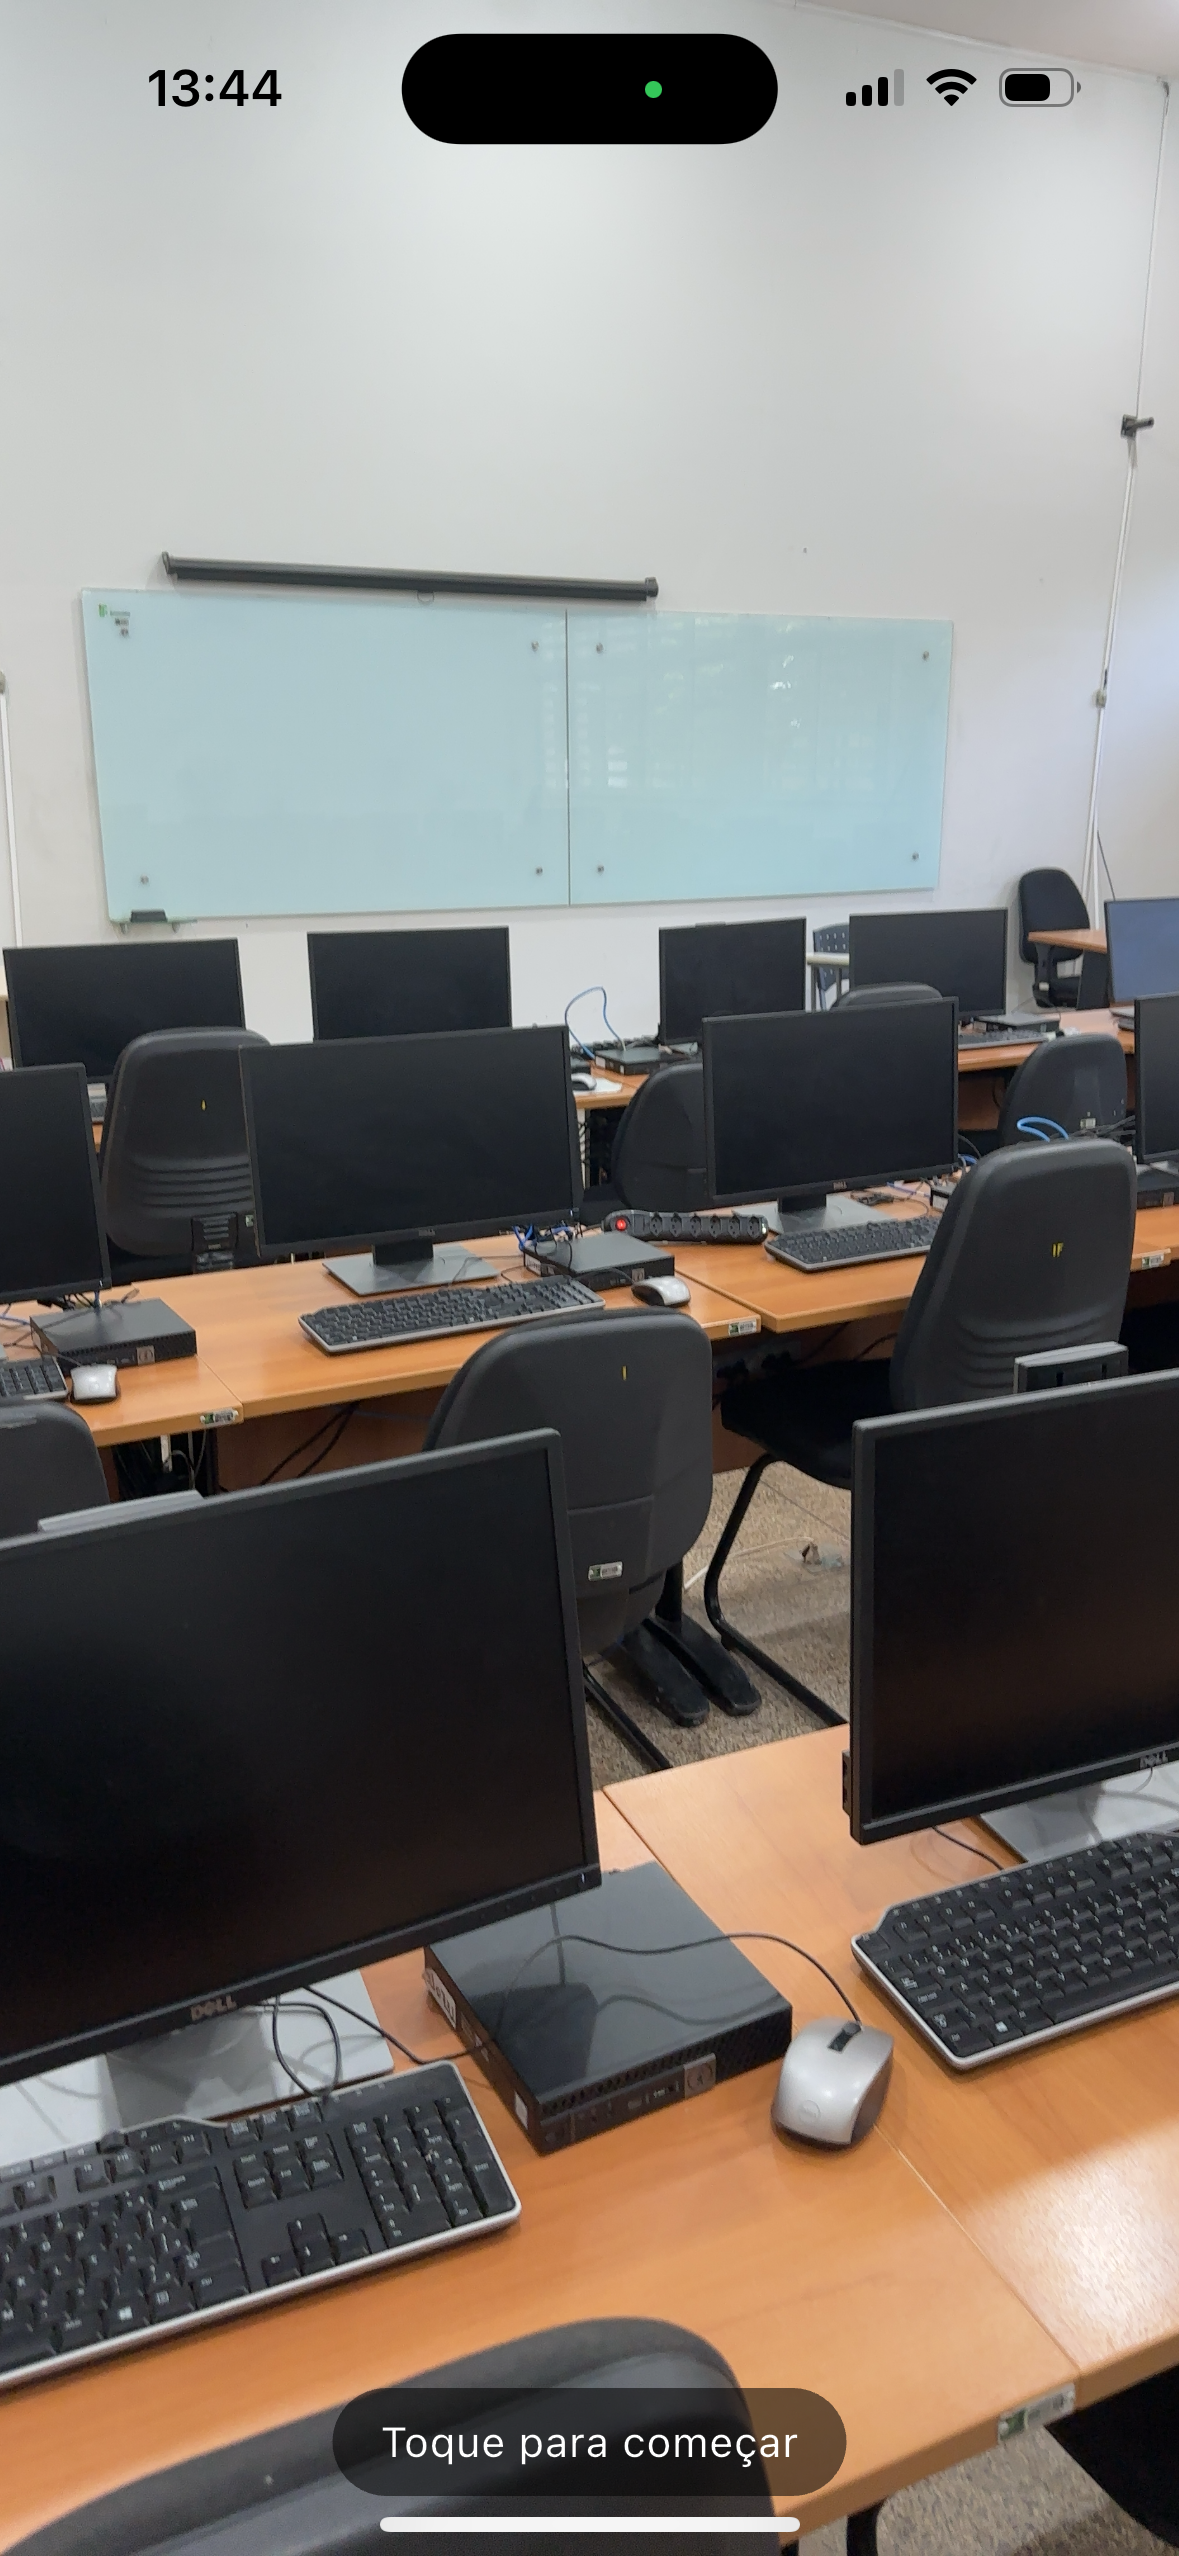
\includegraphics[width=0.4\linewidth]{imagens/tela-inicial.png}
     \label{fig:10}
     \caption*{\textbf{Fonte:} Elaborado pelo Autor (2025)}
\end{figure}

\begin{figure}[!ht]
     \caption{Tela após o início da gravação e captura da imagem}
     \centering
     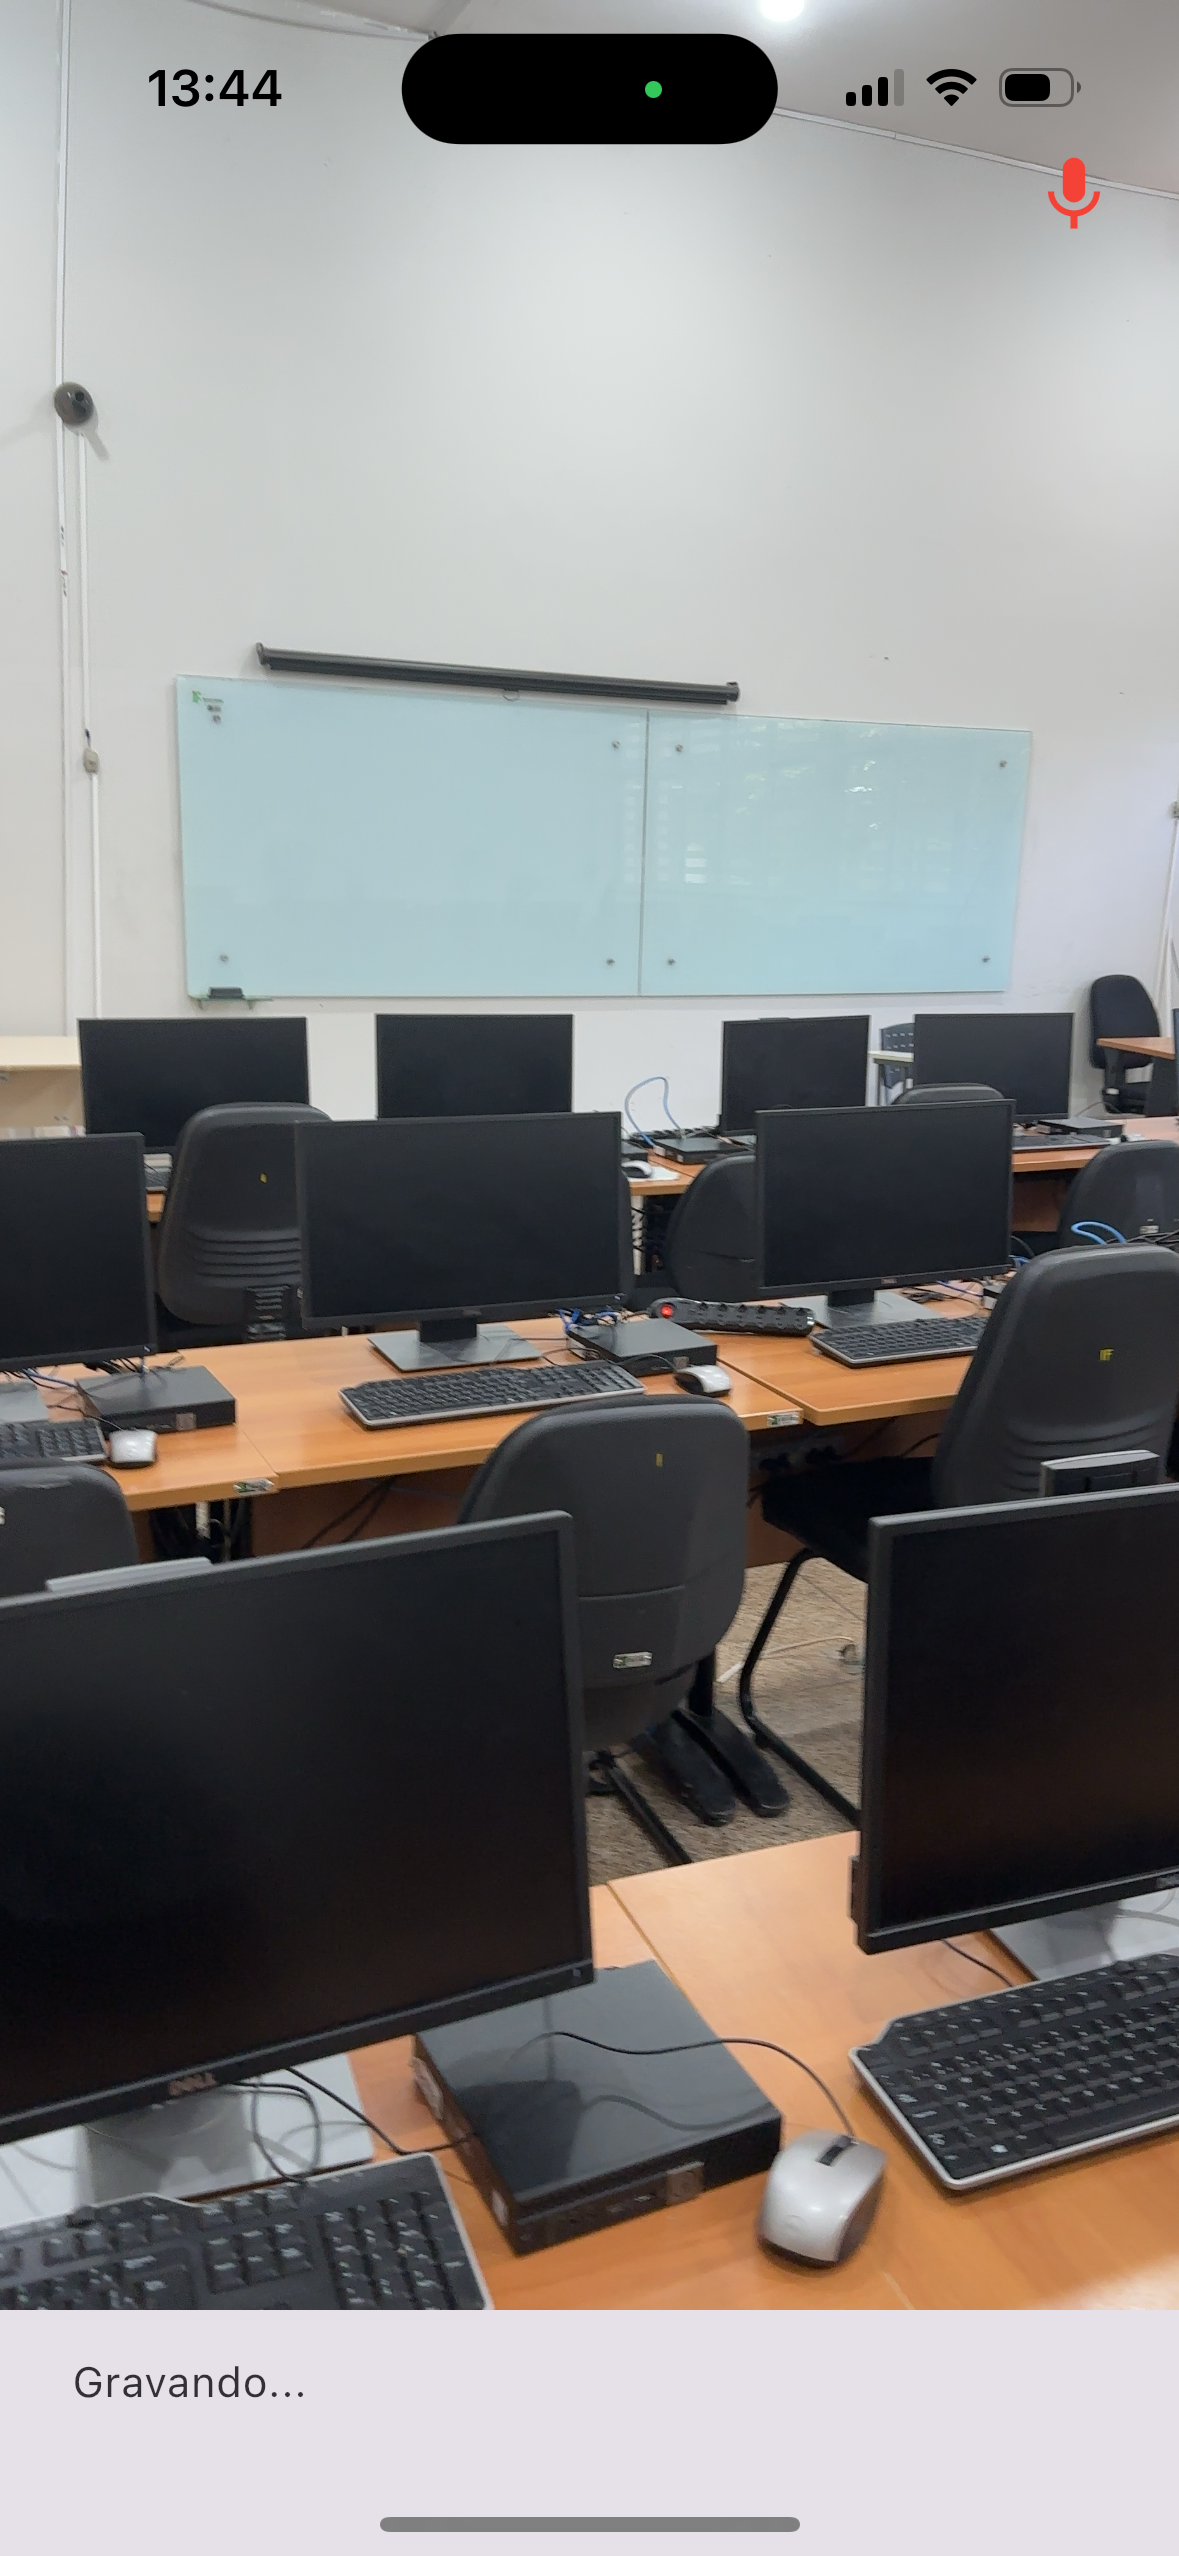
\includegraphics[width=0.4\linewidth]{imagens/gravacao.png}
     \label{fig:11}
     \caption*{\textbf{Fonte:} Elaborado pelo Autor (2025)}
\end{figure}

\begin{figure}[!ht]
     \caption{Tela após o segundo toque e envio da solicitação à API}
     \centering
     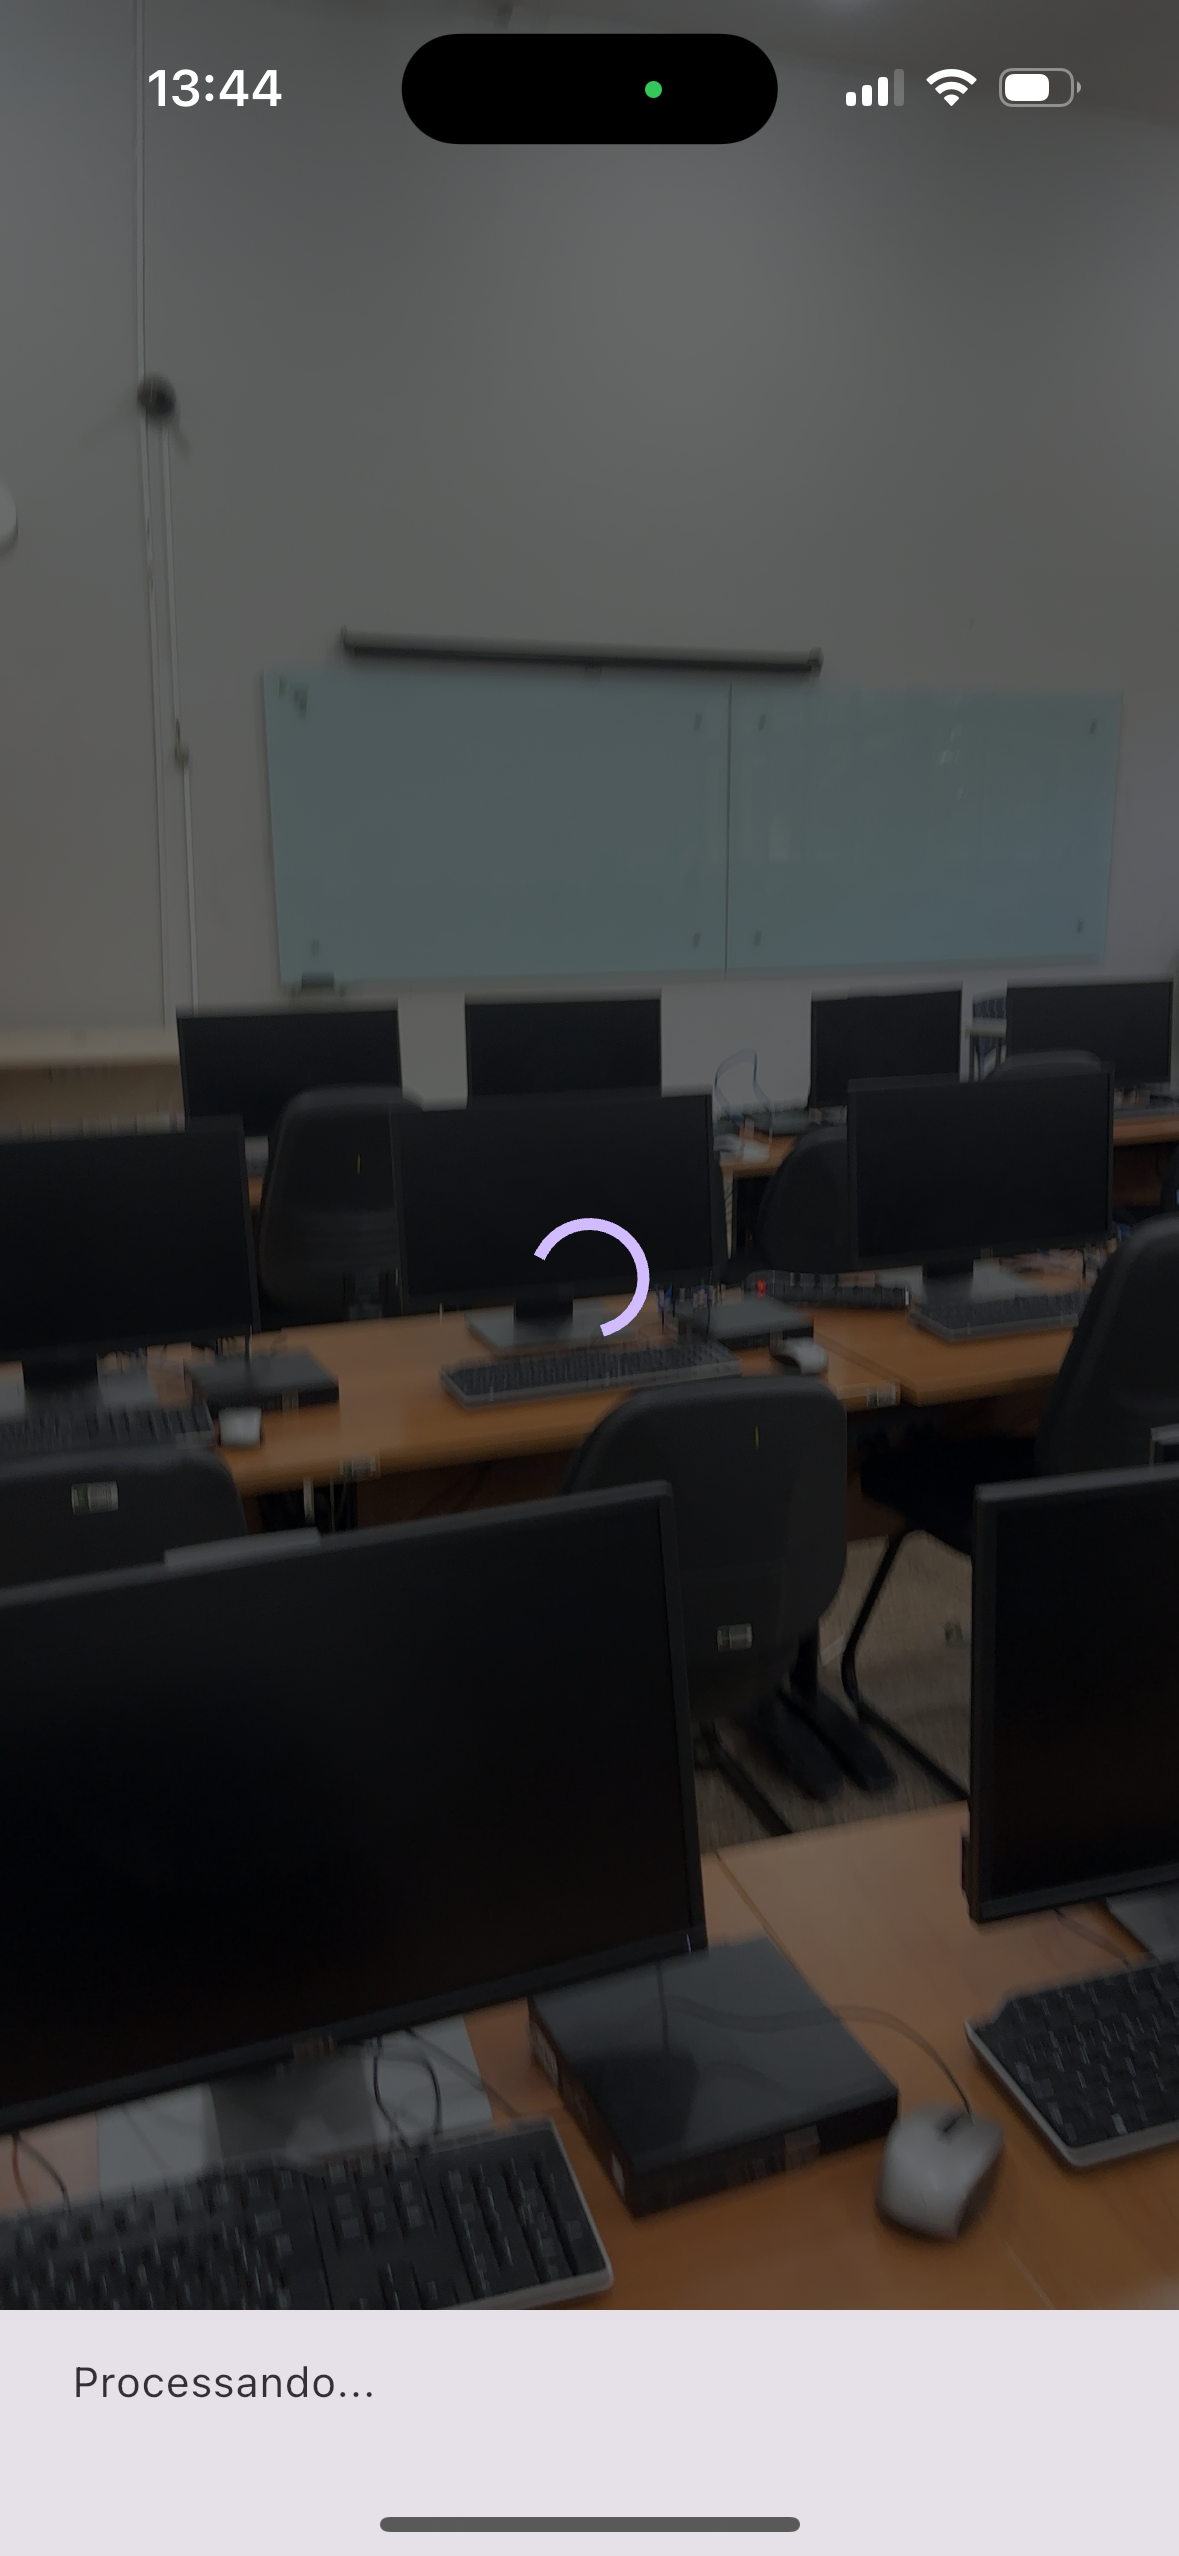
\includegraphics[width=0.4\linewidth]{imagens/requisicao.png}
     \label{fig:12}
     \caption*{\textbf{Fonte:} Elaborado pelo Autor (2025)}
\end{figure}

\subsubsection{Desempenho e Qualidade das Descrições}

Os testes realizados em diversos cenários — ambientes internos com baixa iluminação, áreas externas sob luz natural intensa, presença de múltiplos objetos — corroboraram a eficiência do \lstinline{Qwen2.5-VL-7B-Instruct} apontada no \textit{benchmark}. Em termos de desempenho, constatou-se que o tempo entre a captura da imagem e a transmissão do áudio final ao usuário permaneceu baixo, viabilizando a sensação de tempo real. Esse resultado decorre, em grande parte, da menor latência do modelo escolhido em comparação com os demais modelos avaliados.

Quanto à qualidade das descrições, observou-se que o \lstinline{Qwen2.5-VL-7B-Instruct} geralmente forneceu legendas coerentes e detalhadas. Mesmo em situações mais complexas, a identificação dos elementos principais se manteve satisfatória, embora algumas descrições possam omitir detalhes ou interpretar incorretamente alguns objetos e situações presentes na imagem. Na maioria dos testes, porém, o conteúdo foi suficiente para dar ao usuário uma noção clara do ambiente, alinhando-se ao objetivo assistivo proposto.

Pode-se avaliar o resultado final tomando como exemplo a imagem retirada da Figura 10, onde foi realizado o processo inicial da captura da imagem e gravação do áudio, conforme evidenciam as Figuras \ref{fig:11} e \ref{fig:12}. Neste caso, ao ser enviada a solicitação à API, o modelo realizou a inferência e retornou a seguinte resposta: "A imagem mostra uma sala de computadores com várias mesas dispostas lado a lado. Cada mesa tem um monitor de computador, um teclado e um mouse. À esquerda, há uma lousa branca com quadros pretos. O ambiente parece ser uma sala de aula ou um centro de aprendizagem. Não há riscos visíveis na imagem."

\subsubsection{Acessibilidade e Integração}

A utilização contínua do TTS durante todo o ciclo de uso garante que o sistema seja efetivamente acessível, possibilitando que o usuário receba instruções e descrições em áudio sem a necessidade de auxílio visual ou suporte adicional. Paralelamente, a API abstrai a complexidade do modelo de IA, de modo que o aplicativo em Flutter se mantém leve e simples de operar em qualquer dispositivo móvel compatível.

Com esse design modular, a robustez do servidor e do modelo, incluindo possíveis evoluções ou substituições futuras, não altera a experiência de quem utiliza o aplicativo. Isso potencializa a escalabilidade e a flexibilidade do sistema, contribuindo para que a solução possa ser continuamente atualizada sem comprometer o foco assistivo.

\subsubsection{Síntese dos Resultados}

A avaliação prática do sistema revelou três aspectos fundamentais para o sucesso da proposta. Em primeiro lugar, a baixa latência efetiva proporcionou respostas ágeis, fator indispensável em aplicações assistivas que demandam \textit{feedback} quase imediato. Em segundo lugar, as descrições fornecidas pelo \lstinline{Qwen2.5-VL-7B-Instruct} mostraram-se suficientemente coerentes para oferecer ao usuário uma compreensão geral do ambiente, cumprindo com êxito o papel de fornecer legendas informativas na maioria dos cenários testados.

Por fim, a integração do TTS ao longo de todo o fluxo de interação evidenciou o potencial inclusivo do protótipo, tornando o sistema acessível e viabilizando a utilização independente por pessoas com deficiência visual. Assim, conclui-se que o protótipo não apenas se apoia em um modelo de IA robusto, mas também adota uma interface voltada ao público-alvo, garantindo praticidade, rapidez e uma experiência de uso imersiva.

\section{Análise Crítica dos Resultados}

A avaliação prática do protótipo integrado — aplicativo Flutter, API em Python e modelo \lstinline{Qwen2.5-VL-7B-Instruct} — evidenciou que a escolha do modelo se revelou eficaz tanto no quesito latência quanto na qualidade das descrições. A baixa latência possibilitou que o usuário recebesse as informações de modo quase imediato, fator imprescindível para aplicações assistivas. Nesse sentido, o \lstinline{Qwen2.5} provou ser uma opção mais equilibrada do que os demais modelos testados, que enfrentaram problemas de alto consumo de memória ou tempos de resposta excessivos.

Do ponto de vista do TTS, a experiência de uso foi satisfatória. A adoção de mensagens de áudio em cada etapa reduziu a dependência de interfaces visuais, assegurando que o protótipo estivesse plenamente alinhado aos princípios de acessibilidade. Ainda assim, é importante salientar que a precisão das descrições pode variar em cenários de maior complexidade visual, ou quando a iluminação é precária. Nessas situações, o modelo pode apresentar falhas pontuais de identificação ou omissões. Não obstante, no conjunto das avaliações, o sistema cumpriu seu objetivo de prover ao usuário uma visão geral do ambiente, demonstrando o potencial de integração entre tecnologias de visão computacional, modelos de linguagem e aplicações mobile para promover inclusão digital.

O projeto também revela um \textit{trade-off} claro entre desempenho e robustez. Embora o \lstinline{Qwen2.5} ofereça respostas confiáveis em tempo razoável, modelos maiores (como o \lstinline{Llama-3.2-11B-Vision-Instruct}) poderiam, em teoria, gerar descrições mais ricas, porém à custa de maior latência e requisitos de \textit{hardware}. A escolha final recai, pois, sobre a necessidade de um equilíbrio entre esses fatores, priorizando a experiência do usuário com deficiência visual, que requer fluidez e respostas rápidas para contextos do cotidiano.

\section{Limitações}

Apesar dos resultados promissores, o trabalho apresenta algumas limitações que precisam ser consideradas. Em primeiro lugar, há a dependência de uma conexão com a internet para que o protótipo possa se comunicar com o servidor remoto, onde está hospedado o modelo de IA. Em regiões com acesso precário ou instável à rede, essa característica tende a aumentar a latência ou até mesmo inviabilizar o funcionamento do sistema. Além disso, a execução de testes com centenas de imagens revelou que a capacidade de GPU disponível foi ocasionalmente excedida, evidenciando a necessidade de recursos computacionais mais robustos ou de técnicas mais avançadas de otimização, como a quantização mais avançada ou distribuição de carga em múltiplas instâncias de servidores, para garantir um desempenho consistente em larga escala.

Outro ponto a destacar diz respeito ao comportamento do modelo em cenários de alta complexidade visual. Embora o modelo definido ofereça descrições satisfatórias na maioria das situações, imagens muito sobrecarregadas de detalhes ou mal iluminadas podem resultar em legendas incompletas ou confusas, exigindo técnicas adicionais de pré-processamento de imagens ou modelos especializados em tais condições. Também vale ressaltar que, apesar de os testes internos terem indicado uma boa experiência, não foram realizadas avaliações extensivas com um público diversificado de pessoas com deficiência visual, de modo que a validação do protótipo em cenários reais de mobilidade e diferentes perfis de usuários permanece como uma lacuna a ser suprida em trabalhos futuros.

Por fim, é importante considerar que o sistema desenvolvido se configura como um protótipo experimental, cujo foco principal foi demonstrar a viabilidade de integrar um modelo de IA relativamente robusto em um aplicativo destinado à acessibilidade. Assim, essas limitações não anulam o mérito dos resultados obtidos, mas apontam caminhos concretos para avanços, seja no aprimoramento da infraestrutura de processamento, seja na incorporação de técnicas adicionais de otimização e na ampliação dos testes de campo com usuários finais.

